%!TEX root = ../../../_main.tex
\subsection{Residuums}
\label{sec:twisted-involutions-residuums}

\begin{defi}
	\typedlabel{defi:residuum}
	Let $w \in W$ and $I \subseteq S$ be a subset of generators. Then we define
	$$ wC_I := \{ w \ul s_1 \ldots \ul s_k : k \in \nn_0, s_i \in S \} $$
	as the \defword{$I$-residuum} of $w$ or just \defword{residuum}. To emphasize the size of $I$, say $|I| = n$, we also speak of a \defword{rank-$n$-residuum}.
\end{defi}

\begin{exam}
	Let $w \in W$. Then $wC_\emptyset = \{ w \}$ and $wC_S = \ti{\theta}$.
\end{exam}

\begin{lemm}
	\typedlabel{lemm:all-elements-of-one-residuum-yield-the-same-residuum}
	Let $w \in W$ and $I \subset S$. If $v \in wC_I$, then $vC_I = wC_I$.

	\begin{proof}
		Suppose $v \in wC_I$. Then $v = w \ul s_1 \ldots \ul s_n$ for some $s_i \in I$. Suppose $u = w \ul t_1 \ldots \ul t_m \in wC_I$ is any other element in $wC_I$ with $t_i \in I$. Then
		$$ u = w \ul t_1 \ldots \ul t_m = (v \ul s_n \ldots \ul s_1) \ul t_1 \ldots \ul t_m $$
		and so $u \in vC_I$. This yields $wC_I \subset vC_I$. Since $w \in vC_I$ we can swap $v$ and $w$ to get the other inclusion.
	\end{proof}
\end{lemm}

\begin{coro}
	Let $v, w \in W$ and $I \subset S$. Then either $vC_I \cap wC_I = \emptyset$ or $vC_I = wC_I$.

	\begin{proof}
		Immediately follows from \ref{lemm:all-elements-of-one-residuum-yield-the-same-residuum}.
	\end{proof}
\end{coro}

\begin{prop}
	\typedlabel{prop:residuums-have-unique-wk-theta-minimal-element}
	\theocite{Lemma 5.6}{hultman:comb-twisted-invo}
	Let $w \in \ti{\theta}$, $I \subseteq S$ be a set of generators. Then there exists a unique element $w_0 \in wC_I$ with $w_0 \preceq w_0 \ul s$ for all $s \in I$.

	\begin{proof}
		Suppose there is no such element. Then for each $w \in wC_I$ we can find a $s \in I$ with $w' = w \ul s \preceq w$ and $e' \in wC_I$. By repetition of \ref{prop:deletion-property-for-twisted-expressions} we get, that $e \in wC_I$, but $e$ has the property, which we assumed, that no element in $wC_I$ has. Hence there must be at least one such element. Now suppose there are two distinct elements $u,v$ with the desired property. Note that this means, that $u$ and $w$ have no reduced twisted expression ending with some $\ul s \in I$. Let $v$ have a reduced twisted expression $v = \ul s_1 \ldots \ul s_k$. Since $u$ and $v$ are both in $wC_I$ there must be a twisted $v$-expression for $u$
		$$ u = v \ul s_{k+1} \ldots \ul s_{k+l} = \ul s_1 \ldots \ul s_{k+l} $$
		with $s_n \in I$ for $k+1 \leq n \leq k+l$. This twisted expression cannot be reduced, since it ends with $\ul s_{k+l} \in I$. Then \ref{prop:deletion-property-for-twisted-expressions} yields that this twisted expression contains a reduced twisted subexpression for $u$. It cannot end with $\ul s_n$ for $k+1 \leq n \leq k+l$. Hence, it is a twisted subexpression of $\ul s_1 \ldots \ul s_k = v$, too. So $u \leq v$ by \ref{theo:bruhat-subexpression-characterization}. Because of symmetry we have $v \leq u$ and so $u = v$, contradicting to our assumption $u \neq v$.
	\end{proof}
\end{prop}

\begin{coro}
	\typedlabel{coro:residuums-have-unique-minimal-element}
	Let $w \in \ti{\theta}$, $I \subseteq S$ be a set of generators and let $\rho_{min} := \min \{ \rho(v) : v \in wC_I \}$ be the minimal twisted length within the residuum $wC_I$. Then there is a unique element $w_{min} \in wC_I$ with $\rho(w_{min}) = \rho_{min}$. We denote this element by $\min(w,I)$.

	\begin{proof}
		The minimal rank $\rho_{min}$ exists, since the image of $\rho$ is in $\nn_0$, which is well-ordered, and $wC_I \neq \emptyset$. Suppose we have an element $w_{min}$ with $\rho(w_{min}) = \rho_{min}$. This means, that in particular all $w_{min} \ul s$ with $s \in I$ must be of larger twisted length, i.e. $w_{min} < w_{min} \ul s$ for all $s \in I$. With \ref{prop:residuums-have-unique-wk-theta-minimal-element} this element must be unique.
	\end{proof}
\end{coro}

We proceed with some properties of rank-2-residuums. Our interest in these residuums stems from the fact, that their properties are needed later in Section \ref{sec:twisted-involutions-algorithms} to construct an effective algorithm for calculating the twisted weak ordering, i.e. calculating the Hasse diagram of $Wk(\theta)$ for arbitrary Coxeter systems $(W,S)$ and Coxeter system automorphisms $\theta$.

\begin{defi}
	Let $s,t \in S$ be two distinct generators. We define:
	$$[\ul s \ul t]^n :=
	\begin{cases}
	(\ul s \ul t)^{\frac{n}{2}} & n \textrm{ even}, \\
	(\ul s \ul t)^{\frac{n-1}{2}} \ul s & n \textrm{ odd}. 
	\end{cases}$$
\end{defi}

This definition allows us to express rank-2-residuums differently. Suppose we have an element $w \in \ti{\theta}$ and two distinct generators $s,t \in S$. Thanks to \ref{lemm:all-elements-of-one-residuum-yield-the-same-residuum} and \ref{coro:residuums-have-unique-minimal-element} we can assume, that $w = min(w,\{s,t\})$. Then
$$ wC_{\{s,t\}} = \{ w \} \ \cup \ \{ w [\ul s \ul t]^n : n \in \nn \} \ \cup \ \{ w [\ul t \ul s]^n : n \in \nn \}. $$
This encourages the following definition.

\begin{defi}
	Let $w \in \ti{\theta}$ and let $s,t \in S$ be two distinct generators. Suppose $w = min(w,\{s,t\})$. Then we call $\{ w [\ul s \ul t]^n : n \in \nn \}$ the \defword{$s$-branch} and $\{ w [\ul t \ul s]^n : n \in \nn \}$ the \defword{$t$-branch} of $wC_{\{s,t\}}$.
\end{defi}

One question arises immediately: Are the $s$- and the $t$-branch disjoint? With the following propositions, corollaries and lemmas we will get a much better idea of the structure of rank-2-residuums and answer this question.

\begin{prop}
	\typedlabel{prop:rank-2-residuums-are-convex}
	Let $w \in W$ and let $s,t \in S$ be two distinct generators. Without loss of generality suppose $w = \min(w, \{s,t\})$. If there is a $v \in wC_{\{s,t\}}$ with $v \ul s \prec v$ and $v \ul t \prec v$, then it is unique with this property in $wC_{\{s,t\}}$. Hence $wC_{\{s,t\}}$ consists of two geodesics from $w$ to $v$ intersecting only in these two elements. Else, the $s$- and $t$-branch are disjoint, strictly ascending in twisted length and of infinite size.

	\begin{proof}
		Suppose there is a $v$ in the $s$-branch with $v \ul s \prec v$ and $v \ul t \prec v$, say $v = w[\ul s \ul t]^n$ and $n$ is minimal with this property. Because of the uniqueness of a minimal element from \ref{prop:residuums-have-unique-wk-theta-minimal-element} we have $w[\ul s \ul t]^{m+1} \prec w[\ul s \ul t]^m$ for all $m \in \nn$ with $n \leq m \leq 2n - 1$. With the same argument we have $w[\ul s \ul t]^{2n} = w$. If no such $v$ exists, then the $s$- and $t$-branch must be disjoint, strictly ascending in twisted length and so of infinite size.
	\end{proof}
\end{prop}

\begin{prop}
	\typedlabel{prop:onesided-operations-only-at-top-or-bottom-end-of-twocycle}
	Let $w \in S$ and $s,t \in S$ be two distinct generators. If $\ul s$ acts by multiplications on $w$ and $w \ul s \prec w$, then either $w \ul s \ul t \prec w \ul s$ or $w \ul t \succ w$.

	\begin{proof}
		We have $\theta(s)ws = w$ and $s \in D_R(w)$, hence $w \ul s \leq w$. If $t \notin D_R(w)$ or $t \in D_R(w \ul s)$, then we are done. In return suppose $t \in D_R(w)$ and $t \notin D_R(w \ul s)$. Then we have $w \ul t \leq w$ and $w \ul s \leq w \ul s \ul t$. With the second part of \ref{lemm:lifting-property-for-ul-s} we conclude $(w \ul s \ul t) \ul t \leq w \ul t$. This yields
		$$ ws = w \ul s = (w \ul s \ul t) \ul t \leq w \ul t. $$
		Since $l(w) - 1 = l(w \ul s) \leq l(w \ul t) < l(w)$ we have $w \ul t = wt$, hence $ws \leq wt$. But $s,t \in D_R(w)$ and so $l(ws) = l(wt)$ and $ws = wt$, too. Therefore $s = t$, contradicting our assumption of two distinct generators.
	\end{proof}
\end{prop}

\begin{coro}
	\typedlabel{coro:onesided-operations-only-at-top-or-bottom-end-of-twocycle}
	Let $w \in S$ and let $s,t \in S$ be two distinct generators. If $w$ is neither $\min(w,\{s,t\})$, nor a maximal element in $wC_{\{s,t\}}$, then both $\ul s$ and $\ul t$ act by twisted conjugation on $w$.

	\begin{proof}
		Follows immediately from \ref{prop:onesided-operations-only-at-top-or-bottom-end-of-twocycle}.
	\end{proof}
\end{coro}

\begin{lemm}
	\typedlabel{lemm:one-both-sided-action-symmetric-in-rank-2-residuums}
	Let $s,t \in S$ be two distinct generators and $w \in S$ with $w = min(w,\{s,t\})$. Suppose $v \in wC_{\{s,t\}}$ with $v \ul s \prec v$ and $v \ul t \prec v$. Then the twisted conjugations and mulitplications are distributed axisymmetrically or pointsymmetrically like in Figure \ref{fig:dist-one-bothsided-actions-in-rank-2-residuum}.

	\begin{figure}[ht]
		\centering
		\input{resources/tikz/one-bothsided-symmetry-0000}
		\input{resources/tikz/one-bothsided-symmetry-1111}
		\input{resources/tikz/one-bothsided-symmetry-1100}
		\input{resources/tikz/one-bothsided-symmetry-0011}
		%!TEX root = ../../_main.tex
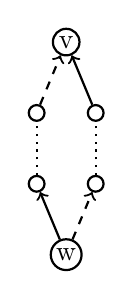
\begin{tikzpicture}[scale=1,bend angle=10]
\newcommand{\xspace}{1}
\newcommand{\yspace}{0.6}
\tikzstyle{vertex}=[draw,thick,circle,minimum size=2mm,inner sep=1pt]
\tikzstyle{edge}=[thick,->]
\tikzstyle{edge2}=[dotted,thick]
\tikzstyle{onesided}=[edge,dashed]
\tikzstyle{bothsided}=[edge]
\node[vertex] (0) at (\xspace*0,\yspace*0) {w};
\node[vertex] (1) at (\xspace*-0.375,\yspace*1.5) {};
\node[vertex] (2) at (\xspace*0.375,\yspace*1.5) {};
\node[vertex] (3) at (\xspace*-0.375,\yspace*3.0) {};
\node[vertex] (4) at (\xspace*0.375,\yspace*3.0) {};
\node[vertex] (5) at (\xspace*0,\yspace*4.5) {v};
\draw[bothsided] (0) edge (1);
\draw[onesided] (0) edge (2);
\draw[edge2] (1) edge (3);
\draw[edge2] (2) edge (4);
\draw[onesided] (3) edge (5);
\draw[bothsided] (4) edge (5);
\end{tikzpicture}
		\input{resources/tikz/one-bothsided-symmetry-0101}
		\caption{Possible distributions of twisted conjugations and multiplications in finite rank-2-residuums}
		\label{fig:dist-one-bothsided-actions-in-rank-2-residuum}
	\end{figure}

	\begin{proof}
		If $u$ covers $w$, then there are only two edges and the assumption holds. So suppose $wC_{\{s,t\}}$ contains at least four edges. Due to \ref{coro:onesided-operations-only-at-top-or-bottom-end-of-twocycle} the actions by multiplication can only occure next to $w$ and $v$. Hence there are $2^4 = 16$ configurations possible. \ref{prop:geodesics-have-same-count-of-multiplicative-steps} wipes out ten out of the 16 configurations. The remaining are those from Figure \ref{fig:dist-one-bothsided-actions-in-rank-2-residuum}.
	\end{proof}
\end{lemm}

\begin{exam}
	In Figure \ref{fig:a4_s1s3-and-a4_s2s4} we see two Hasse diagrams of $Wk(A_4, \id)$. The left one only contains edges with labels $s_1,s_2$, the middle one only edges with labels $s_1,s_3$ and the right one only edges with labels $s_1,s_4$.
	\begin{figure}[ht]
		\centering
		%!TEX root = ../../_main.tex
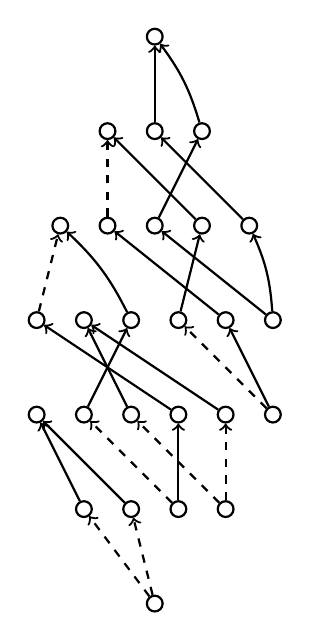
\begin{tikzpicture}[scale=0.8,bend angle=10]
\newcommand{\xspace}{1}
\newcommand{\yspace}{1}
\tikzstyle{vertex}=[draw,thick,circle,minimum size=2mm,inner sep=0pt]
\tikzstyle{edge}=[thick,->]
\tikzstyle{onesided}=[edge,dashed]
\tikzstyle{bothsided}=[edge]
\tikzstyle{unhighlighted}=[]
\tikzstyle{highlighted}=[]
\definecolor{s1color}{RGB}{130,76,253}
\definecolor{s2color}{RGB}{76,253,78}
\definecolor{s3color}{RGB}{253,76,124}
\definecolor{s4color}{RGB}{76,176,253}
\tikzstyle{s1}=[]
\tikzstyle{s2}=[]
\tikzstyle{s3}=[]
\tikzstyle{s4}=[]
\node[vertex,unhighlighted] (0) at (\xspace*0,\yspace*0) {};
\node[vertex,unhighlighted] (1) at (\xspace*-1.125,\yspace*1.5) {};
\node[vertex,unhighlighted] (2) at (\xspace*-0.375,\yspace*1.5) {};
\node[vertex,unhighlighted] (3) at (\xspace*0.375,\yspace*1.5) {};
\node[vertex,unhighlighted] (4) at (\xspace*1.125,\yspace*1.5) {};
\node[vertex,unhighlighted] (5) at (\xspace*-1.875,\yspace*3) {};
\node[vertex,unhighlighted] (6) at (\xspace*-1.125,\yspace*3) {};
\node[vertex,unhighlighted] (7) at (\xspace*-0.375,\yspace*3) {};
\node[vertex,unhighlighted] (8) at (\xspace*0.375,\yspace*3) {};
\node[vertex,unhighlighted] (9) at (\xspace*1.125,\yspace*3) {};
\node[vertex,unhighlighted] (10) at (\xspace*1.875,\yspace*3) {};
\node[vertex,unhighlighted] (11) at (\xspace*-1.875,\yspace*4.5) {};
\node[vertex,unhighlighted] (12) at (\xspace*-1.125,\yspace*4.5) {};
\node[vertex,unhighlighted] (13) at (\xspace*-0.375,\yspace*4.5) {};
\node[vertex,unhighlighted] (14) at (\xspace*0.375,\yspace*4.5) {};
\node[vertex,unhighlighted] (15) at (\xspace*1.125,\yspace*4.5) {};
\node[vertex,unhighlighted] (16) at (\xspace*1.875,\yspace*4.5) {};
\node[vertex,unhighlighted] (17) at (\xspace*-1.5,\yspace*6) {};
\node[vertex,unhighlighted] (18) at (\xspace*-0.75,\yspace*6) {};
\node[vertex,unhighlighted] (19) at (\xspace*0,\yspace*6) {};
\node[vertex,unhighlighted] (20) at (\xspace*0.75,\yspace*6) {};
\node[vertex,unhighlighted] (21) at (\xspace*1.5,\yspace*6) {};
\node[vertex,unhighlighted] (22) at (\xspace*-0.75,\yspace*7.5) {};
\node[vertex,unhighlighted] (23) at (\xspace*0,\yspace*7.5) {};
\node[vertex,unhighlighted] (24) at (\xspace*0.75,\yspace*7.5) {};
\node[vertex,unhighlighted] (25) at (\xspace*0,\yspace*9) {};
\draw[s1,onesided,unhighlighted] (0) edge (1);
\draw[s2,onesided,unhighlighted] (0) edge (2);
\draw[s2,bothsided,unhighlighted] (1) edge (5);
\draw[s1,bothsided,unhighlighted] (2) edge (5);
\draw[s1,onesided,unhighlighted] (3) edge (6);
\draw[s2,bothsided,unhighlighted] (3) edge (8);
\draw[s1,onesided,unhighlighted] (4) edge (7);
\draw[s2,onesided,unhighlighted] (4) edge (9);
\draw[s2,bothsided,unhighlighted] (6) edge (13);
\draw[s2,bothsided,unhighlighted] (7) edge (12);
\draw[s1,bothsided,unhighlighted] (8) edge (11);
\draw[s1,bothsided,unhighlighted] (9) edge (12);
\draw[s1,onesided,unhighlighted] (10) edge (14);
\draw[s2,bothsided,unhighlighted] (10) edge (15);
\draw[s2,onesided,unhighlighted] (11) edge (17);
\draw[s1,bothsided,unhighlighted,bend right] (13) edge (17);
\draw[s2,bothsided,unhighlighted] (14) edge (20);
\draw[s1,bothsided,unhighlighted] (15) edge (18);
\draw[s1,bothsided,unhighlighted] (16) edge (19);
\draw[s2,bothsided,unhighlighted,bend right] (16) edge (21);
\draw[s2,onesided,unhighlighted] (18) edge (22);
\draw[s2,bothsided,unhighlighted] (19) edge (24);
\draw[s1,bothsided,unhighlighted] (20) edge (22);
\draw[s1,bothsided,unhighlighted] (21) edge (23);
\draw[s2,bothsided,unhighlighted] (23) edge (25);
\draw[s1,bothsided,unhighlighted,bend right] (24) edge (25);
\end{tikzpicture}
		\quad \quad
		%!TEX root = ../../_main.tex
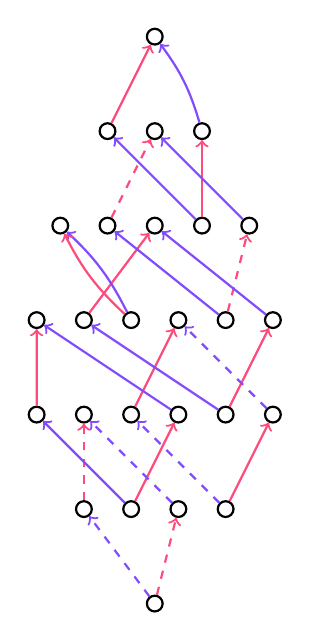
\begin{tikzpicture}[scale=0.8,bend angle=10]
\newcommand{\xspace}{1}
\newcommand{\yspace}{1}
\tikzstyle{vertex}=[draw,thick,circle,minimum size=2mm,inner sep=0pt]
\tikzstyle{edge}=[thick,->]
\tikzstyle{onesided}=[edge,dashed]
\tikzstyle{bothsided}=[edge]
\tikzstyle{unhighlighted}=[]
\tikzstyle{highlighted}=[]
\definecolor{s1color}{RGB}{130,76,253}
\definecolor{s2color}{RGB}{76,253,78}
\definecolor{s3color}{RGB}{253,76,124}
\definecolor{s4color}{RGB}{76,176,253}
\tikzstyle{s1}=[s1color]
\tikzstyle{s2}=[s2color]
\tikzstyle{s3}=[s3color]
\tikzstyle{s4}=[s4color]
\node[vertex,unhighlighted] (0) at (\xspace*0,\yspace*0) {};
\node[vertex,unhighlighted] (1) at (\xspace*-1.125,\yspace*1.5) {};
\node[vertex,unhighlighted] (2) at (\xspace*-0.375,\yspace*1.5) {};
\node[vertex,unhighlighted] (3) at (\xspace*0.375,\yspace*1.5) {};
\node[vertex,unhighlighted] (4) at (\xspace*1.125,\yspace*1.5) {};
\node[vertex,unhighlighted] (5) at (\xspace*-1.875,\yspace*3) {};
\node[vertex,unhighlighted] (6) at (\xspace*-1.125,\yspace*3) {};
\node[vertex,unhighlighted] (7) at (\xspace*-0.375,\yspace*3) {};
\node[vertex,unhighlighted] (8) at (\xspace*0.375,\yspace*3) {};
\node[vertex,unhighlighted] (9) at (\xspace*1.125,\yspace*3) {};
\node[vertex,unhighlighted] (10) at (\xspace*1.875,\yspace*3) {};
\node[vertex,unhighlighted] (11) at (\xspace*-1.875,\yspace*4.5) {};
\node[vertex,unhighlighted] (12) at (\xspace*-1.125,\yspace*4.5) {};
\node[vertex,unhighlighted] (13) at (\xspace*-0.375,\yspace*4.5) {};
\node[vertex,unhighlighted] (14) at (\xspace*0.375,\yspace*4.5) {};
\node[vertex,unhighlighted] (15) at (\xspace*1.125,\yspace*4.5) {};
\node[vertex,unhighlighted] (16) at (\xspace*1.875,\yspace*4.5) {};
\node[vertex,unhighlighted] (17) at (\xspace*-1.5,\yspace*6) {};
\node[vertex,unhighlighted] (18) at (\xspace*-0.75,\yspace*6) {};
\node[vertex,unhighlighted] (19) at (\xspace*0,\yspace*6) {};
\node[vertex,unhighlighted] (20) at (\xspace*0.75,\yspace*6) {};
\node[vertex,unhighlighted] (21) at (\xspace*1.5,\yspace*6) {};
\node[vertex,unhighlighted] (22) at (\xspace*-0.75,\yspace*7.5) {};
\node[vertex,unhighlighted] (23) at (\xspace*0,\yspace*7.5) {};
\node[vertex,unhighlighted] (24) at (\xspace*0.75,\yspace*7.5) {};
\node[vertex,unhighlighted] (25) at (\xspace*0,\yspace*9) {};
\draw[s1,onesided,unhighlighted] (0) edge (1);
\draw[s3,onesided,unhighlighted] (0) edge (3);
\draw[s3,onesided,unhighlighted] (1) edge (6);
\draw[s1,bothsided,unhighlighted] (2) edge (5);
\draw[s3,bothsided,unhighlighted] (2) edge (8);
\draw[s1,onesided,unhighlighted] (3) edge (6);
\draw[s1,onesided,unhighlighted] (4) edge (7);
\draw[s3,bothsided,unhighlighted] (4) edge (10);
\draw[s3,bothsided,unhighlighted] (5) edge (11);
\draw[s3,bothsided,unhighlighted] (7) edge (14);
\draw[s1,bothsided,unhighlighted] (8) edge (11);
\draw[s1,bothsided,unhighlighted] (9) edge (12);
\draw[s3,bothsided,unhighlighted] (9) edge (16);
\draw[s1,onesided,unhighlighted] (10) edge (14);
\draw[s3,bothsided,unhighlighted] (12) edge (19);
\draw[s1,bothsided,unhighlighted,bend right] (13) edge (17);
\draw[s3,bothsided,unhighlighted,bend left] (13) edge (17);
\draw[s1,bothsided,unhighlighted] (15) edge (18);
\draw[s3,onesided,unhighlighted] (15) edge (21);
\draw[s1,bothsided,unhighlighted] (16) edge (19);
\draw[s3,onesided,unhighlighted] (18) edge (23);
\draw[s1,bothsided,unhighlighted] (20) edge (22);
\draw[s3,bothsided,unhighlighted] (20) edge (24);
\draw[s1,bothsided,unhighlighted] (21) edge (23);
\draw[s3,bothsided,unhighlighted] (22) edge (25);
\draw[s1,bothsided,unhighlighted,bend right] (24) edge (25);
\end{tikzpicture}
		\quad \quad
		\input{resources/tikz/a4_s1s4}
		\caption{Hasse diagrams of $Wk(A_4, \id)$ after removing $s_3,s_4$ edges in the left, $s_2,s_4$ edges in the middle and $s_2,s_3$ edges in the right diagram}
		\label{fig:a4_s1s3-and-a4_s2s4}
	\end{figure}
\end{exam}

\begin{lemm}
	\typedlabel{lemm:max-twisted-circle-height}
	Let $w \in S$, $s,t \in S$ be two distinct generators and $m = \ord(st) < \infty$. Then $|wC_{\{s,t\}}| \leq 2m$.

	\begin{proof}
		Let $w$ be the $Wk$-minimal element and $v$ be the $Wk$-maximal element in our residuum. Due to \ref{lemm:one-both-sided-action-symmetric-in-rank-2-residuums} there are six different cases we have to consider. We handle the cases in Figure~\ref{fig:dist-one-bothsided-actions-in-rank-2-residuum} from left to right:
		\begin{description}
			\item[First:] We have $w (\ul s \ul t)^m = (ts)^m w (st)^m = w$.
			\item[Second:] Due to $\theta(s)w = ws$ and $\theta(t)w = wt$ we have
			$$ w (\ul s \ul t)^{m/2+1} = \theta(\hat t (st)^{m/2-1} \hat s) w (st)^{m/2+1} = w(st)^m = w. $$
			(\todo \ Show that this situation only occurs for even $m$)
			\item[Third:] Again we are in a case, where $\theta(s)w = ws$ and $\theta(t)w = wt$ hold. Hence we have
			$$ w (\ul s \ul t)^{(m+1)/2} = \theta(\hat t (st)^{(m-1)/2} \hat s) w (st)^{(m+1)/2} = w(st)^m = w. $$
			(\todo \ Show that this situation only occurs for odd $m$)
			\item[Fourth:] Analogue to the previous case, if we start from $u$ instead of $w$.
			\item[Fifth:] Suppose $m$ is even. Then we have
			$$ w (\ul s \ul t)^m = \theta(\underbrace{ts \cdots st}_{m-1} \hat s \underbrace{ts \cdots st}_{m-1} \hat s) w (st)^m = \theta(\underbrace{ts \cdots s}_{m-2} \underbrace{s \cdots st}_{m-2}) w = \ldots = w. $$
			If $m$ is odd, then we have the completely analogue situation
			$$ w (\ul s \ul t)^m = \theta(\underbrace{ts \cdots ts}_{m-1} \hat t \underbrace{st \cdots st}_{m-1} \hat s) w (st)^m = \theta(\underbrace{ts \cdots t}_{m-2} \underbrace{t \cdots st}_{m-2}) w = \ldots = w. $$
			\item[Sixth:] Analogue to the previous case due to symmetry.
		\end{description}
		So in all six cases we have $w (\ul s \ul t)^k = w$ for a $k \leq \ord(st)$ and hence the residuum can have at most $2 \cdot \ord(st)$ many distinct elements.
	\end{proof}
\end{lemm}

\begin{prop}
	\typedlabel{prop:rank-2-residuum-minimal-k}
	Let $w \in S$ and $s,t \in S$ be two distinct generators with $\ord(st) < \infty$. Suppose $k \in \nn$ to be the smallest number with $w = w(\ul s \ul t)^k$. Then for any $n \in \nn$ with $w = w(\ul s \ul t)^n$ we have $k \ | \ n$.

	\begin{proof}
		Let $n = qk + r$ for $q \in \nn_0$ and $r \in \{0,\ldots,k-1\}$. Then
		$$ w(\ul s \ul t)^n = w(\ul s \ul t)^{qk+r} = w((\ul s \ul t)^k)^q (\ul s \ul t)^r = w(\ul s \ul t)^r. $$
		For $r > 0$ we would have a contradiction to the minimality of $k$, hence $r = 0$, $q > 0$ and therefore $k \ | \ n$.
	\end{proof}
\end{prop}

\begin{coro}
	\typedlabel{coro:rank-2-residuum-gcd-n-m}
	Let $w \in S$ and $s,t \in S$ be two distinct generators with $w \ul s \neq w \ul t$. Suppose $w = w(\ul s \ul t)^m = w(\ul s \ul t)^n$. Then $\gcd(m,n) > 1$.

	\begin{proof}
		Let $k$ be the same as in \ref{prop:rank-2-residuum-minimal-k}. Since $w \ul s \neq w \ul t$ we have $k > 1$. Both, $k \ | \ n$ and $k \ | \ m$, hence $\gcd(m,n) \geq k > 1$.
	\end{proof}
\end{coro}This constraints the possible size of rank-2-residuums.